%3D Pythagoras - Triangular Prism


\documentclass[tikz,border=10pt]{standalone}
\usepackage{tikz}
\usetikzlibrary{3d, angles, quotes} % for 3d vector calculations

\begin{document}

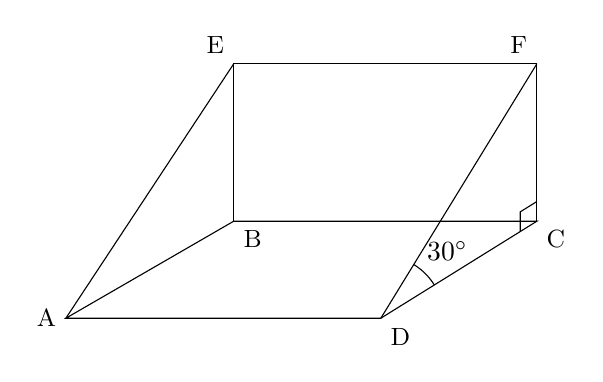
\begin{tikzpicture}[scale=1, transform shape]
    % Define the points of the cube
    \coordinate (A) at (0,0.5,0);
    \coordinate (B) at (0.4,0,-4.5);
    \coordinate (C) at (4.25,0,-4.5);
    \coordinate (D) at (4,0.5,0);
    \coordinate (E) at (0.4,2,-4.5);
    \coordinate (F) at (4.25,2,-4.5);

    % Draw the visible edges of the cube
    \draw (A) -- (B) -- (C) -- (D) -- cycle; % bottom face
    \draw (E) -- (F) -- (C) -- (B) -- cycle; % back face
    \draw (E) -- (A); 
    \draw (F) -- (D);

    % Right angle symbol at D for angle DCF
    \draw pic[draw, angle radius=2.5mm] {right angle=D--C--F};
    \draw pic[draw, angle radius=8mm, angle eccentricity=1.5, "$30^\circ$"] {angle=C--D--F};

    % Place the labels with smaller font size
    \node at (A) [left,font=\small] {A};
    \node at (B) [below right,font=\small] {B};
    \node at (C) [below right,font=\small] {C};
    \node at (D) [below right,font=\small] {D};
    \node at (E) [above left,font=\small] {E};
    \node at (F) [above left,font=\small] {F};
\end{tikzpicture}

\end{document}